\documentclass[tikz,border=6pt]{standalone}
\usepackage{tikz}

\usetikzlibrary{arrows.meta,positioning,fit,calc}

\begin{document}
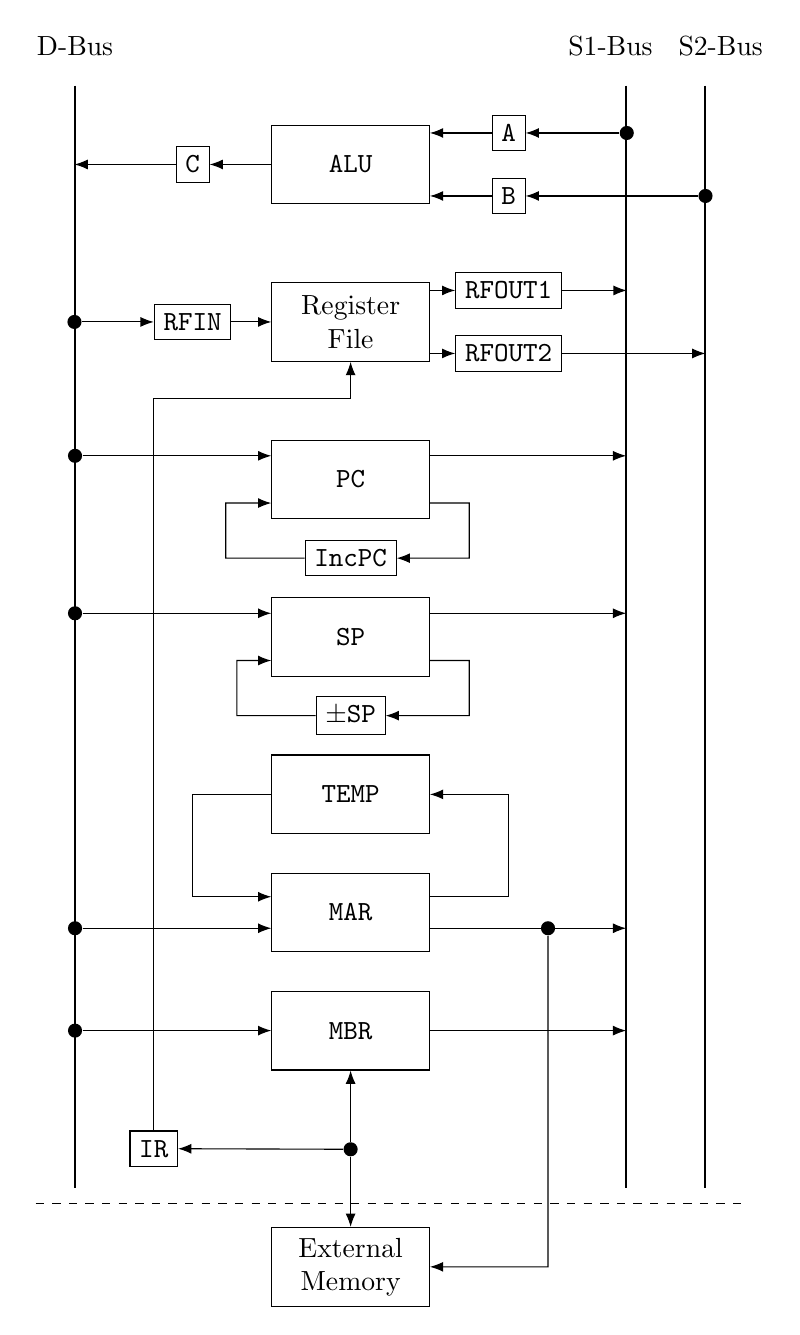
\begin{tikzpicture}[
    box/.style={draw,rounded corners=0pt,minimum width=2cm,minimum height=1cm,align=center},
    textbox/.style={draw,rounded corners=0pt,align=center},
    <-/.style={Latex-},
    ->/.style={-Latex},
    dot/.style={circle,fill,inner sep=1.8pt},
    bus/.style={line width=0.6pt},
]

% ALU components
\node[box] (ALU) at (0,0) {\texttt{ALU}};
\node[textbox] (A) at ($(ALU.east)+(1,0.4)$) {\texttt{A}};
\node[textbox] (B) at ($(ALU.east)+(1,-0.4)$) {\texttt{B}};
\node[textbox] (C) at ($(ALU.west)+(-1,0)$) {\texttt{C}};

% Register File components
\node[box] (RF) at (0,-2) {Register\\File};
\node[textbox] (RFOUT1) at ($(RF.east)+(1,0.4)$) {\texttt{RFOUT1}};
\node[textbox] (RFOUT2) at ($(RF.east)+(1,-0.4)$) {\texttt{RFOUT2}};
\node[textbox] (RFIN) at ($(RF.west)+(-1,0)$) {\texttt{RFIN}};

% PC and IncPC components
\node[box] (PC) at (0,-4) {\texttt{PC}};
\node[textbox] (IncPC) at (0,-5) {\texttt{IncPC}};

% SP components
\node[box] (SP) at (0,-6) {\texttt{SP}};
\node[textbox] (PMSP) at (0,-7) {$\pm$\texttt{SP}};

% Memory components
\node[box] (TEMP) at (0,-8) {\texttt{TEMP}};
\node[box] (MAR) at (0,-9.5) {\texttt{MAR}};
\node[box] (MBR) at (0,-11) {\texttt{MBR}};
\node[box] (EXM) at (0,-14) {External\\Memory};
\node[textbox] (IR) at (-2.5,-12.5) {\texttt{IR}};

% Buses
\draw[bus] (-3.5,1) -- (-3.5,-13);       % D-Bus
\node at (-3.5,1.5) {D-Bus};
\draw[bus] (3.5,1) -- (3.5,-13);         % S1-Bus
\node[align=center] at (3.3,1.5) {S1-Bus};
\draw[bus] (4.5,1) -- (4.5,-13);         % S2-Bus
\node[align=center] at (4.7,1.5) {S2-Bus};

% Dash
\draw[dashed] (-4,-13.2) -- (5,-13.2);

% Connections
% Dots & Coords
\node[dot] (s1_A) at ($(A.center)+(1.5,0)$) {};
\node[dot] (s2_B) at ($(B.center)+(2.5,0)$) {};
\coordinate (d_C) at ($(C.center)+(-1.5,0)$);

\node[dot] (d_RFIN) at ($(RFIN.center)+(-1.5,0)$) {};
\coordinate (s1_RFOUT1) at ($(RFOUT1.center)+(1.5,0)$);
\coordinate (s2_RFOUT2) at ($(RFOUT2.center)+(2.5,0)$);

\node[dot] (d_PC) at ($(PC.center)+(-3.5,0.3)$) {};
\coordinate (s1_PC) at ($(PC.center)+(3.5,0.3)$);

\node[dot] (d_SP) at ($(SP.center)+(-3.5,0.3)$) {};
\coordinate (s1_SP) at ($(SP.center)+(3.5,0.3)$);

\node[dot] (d_MAR) at ($(MAR.center)+(-3.5,-0.2)$) {};
\coordinate (s1_MAR) at ($(MAR.center)+(3.5,-0.2)$);
\node[dot] (d_MBR) at ($(MBR.center)+(-3.5,0)$) {};
\coordinate (s1_MBR) at ($(MBR.center)+(3.5,0)$);

\node[dot] (MAR_EXM) at ($(MAR.east)+(1.5,-0.2)$) {};

\node[dot] (MBR_IR_EXM) at ($(MBR.south)+(0,-1)$) {};

% Arrows
\draw[<-] (d_C) -- (C.west);
\draw[<-] (C.east) -- (ALU.west);
\draw[<-] (ALU.east |- A.west) -- (A.west);
\draw[<-] (ALU.east |- B.west) -- (B.west);
\draw[<-] (A.east) -- (s1_A);
\draw[<-] (B.east) -- (s2_B);

\draw[->] (d_RFIN) -- (RFIN.west);
\draw[->] (RFIN.east) -- (RF.west);
\draw[->] (RF.east |- RFOUT1.west) -- (RFOUT1.west);
\draw[->] (RF.east |- RFOUT2.west) -- (RFOUT2.west);
\draw[->] (RFOUT1.east) -- (s1_RFOUT1);
\draw[->] (RFOUT2.east) -- (s2_RFOUT2);

\draw[->] (d_PC) -- (PC.west |- d_PC);
\draw[->] (PC.east |- d_PC) -- (s1_PC);
\draw[->] (IncPC.west) -- ++(-1,0) -- ++(0,0.7) -- ($(PC.west)+(0,-0.3)$);
\draw[->] ($(PC.east)+(0,-0.3)$) -- ++(0.5,0) -- ++(0,-0.7) -- (IncPC.east);

\draw[->] (d_SP) -- (SP.west |- d_SP);
\draw[->] (SP.east |- d_SP) -- (s1_SP);
\draw[->] (PMSP.west) -- ++(-1,0) -- ++(0,0.7) -- ($(SP.west)+(0,-0.3)$);
\draw[->] ($(SP.east)+(0,-0.3)$) -- ++(0.5,0) -- ++(0,-0.7) -- (PMSP.east);

\draw[->] (TEMP.west) -- ++(-1,0) -- ++(0,-1.3) -- ($(MAR.west)+(0,0.2)$);
\draw[->] ($(MAR.east)+(0,0.2)$) -- ++(1,0) -- ++(0,1.3) -- (TEMP.east);
\draw[->] (d_MAR) -- (MAR.west |- d_MAR);
\draw[->] (MAR.east |- d_MAR) -- (s1_MAR);
\draw[->] (d_MBR) -- (MBR.west);
\draw[->] (MBR.east) -- (s1_MBR);

\draw[->] (MAR_EXM) -- ++(0,-4.3) -- (EXM.east);

\draw[->] (MBR_IR_EXM) -- (MBR.south);
\draw[->] (MBR_IR_EXM) -- (IR.east);
\draw[->] (MBR_IR_EXM) -- (EXM.north);

\draw[->] (IR.north) -- ++(0,9.3) -- ++(2.5,0) -- (RF.south);

\end{tikzpicture}
\end{document}